\begin{figure}[b!]
    \centering
    \begin{subfigure}[b]{0.50\textwidth}
        \centering
        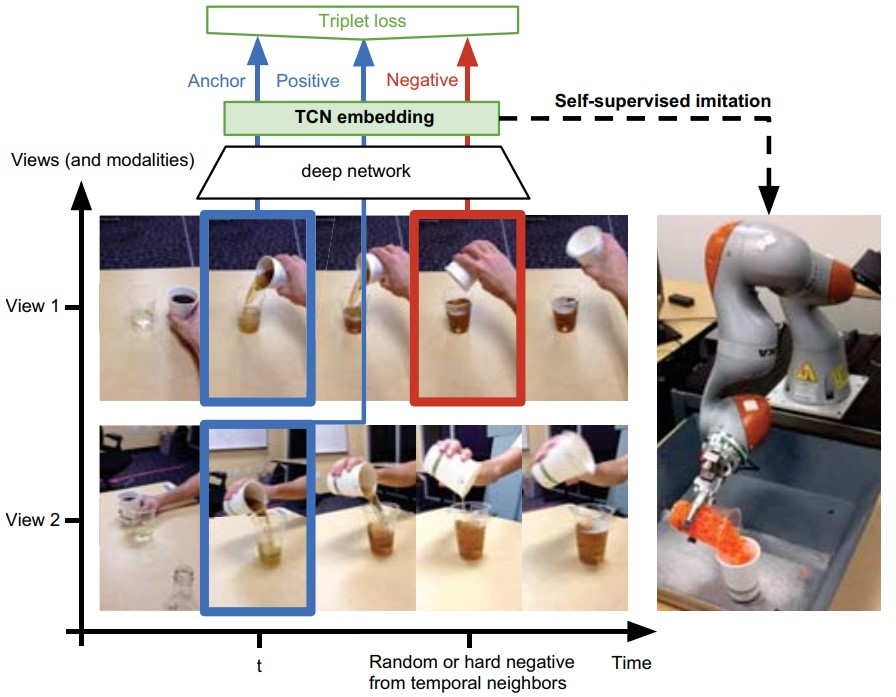
\includegraphics[width=\textwidth]{Figures/images/view_point_mismatch/time-contrastive-network.jpg}
        \caption{Time-Contrastive network, proposed in \cite{sermanet2018time_contrastive}.}
        \label{fig:time_contrastive}
    \end{subfigure}
    \hfill
    \begin{subfigure}[b]{0.45\textwidth}
        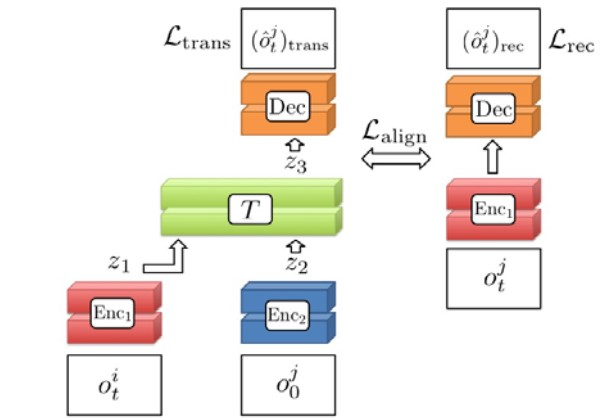
\includegraphics[width=\textwidth]{Figures/images/view_point_mismatch/context-translation-model.jpg}
        \caption{Context-Translation network, proposed in \cite{liu2018imitation_from_observation}}
        \label{fig:context-translation}
    \end{subfigure}
    \caption{Examples of how the mismatch between demonstrator viewpoint and learner viewpoint can be handled.}
    \label{fig:differet_viewpoint}
\end{figure}
